\documentclass[spanish]{beamer}

%Language symbols
\usepackage[spanish]{babel}
\selectlanguage{spanish}
\usepackage[utf8]{inputenc}
\usepackage{verbatim}


\usepackage{graphicx}% http://ctan.org/pkg/graphicx
\usepackage{caption,subcaption}

% Code

\usepackage{listings,textcomp}
\lstset{
  breakatwhitespace,
  language=c++,
  columns=fullflexible,
  keepspaces,
  breaklines,
  tabsize=2, 
  showstringspaces=false,
  extendedchars=true,
  basicstyle=\fontfamily{pcr}\selectfont\scriptsize,
  keywordstyle=\color{orange},
  upquote=true,
  literate={-}{-}1}

%Theme
\usetheme{Madrid}

%Title
\title{Análisis de eficiencia}
\date{\today}
\author{José Antonio Álvarez Ocete}
%Document
\begin{document}

\frame{\titlepage}

\begin{frame}\frametitle{Algoritmos a analizar}

  \begin{itemize}
  \item Burbuja
  \item Insercción
  \item Selección
  \item Mergesort
  \item Quicksort
  \item Heapsort
  \item Floyd 
  \item Hanoi
  \end{itemize}
  
\end{frame}

%
%======================
%

\begin{frame}\frametitle{Algoritmo burbuja}
  \begin{figure}[H]
    \centering   
        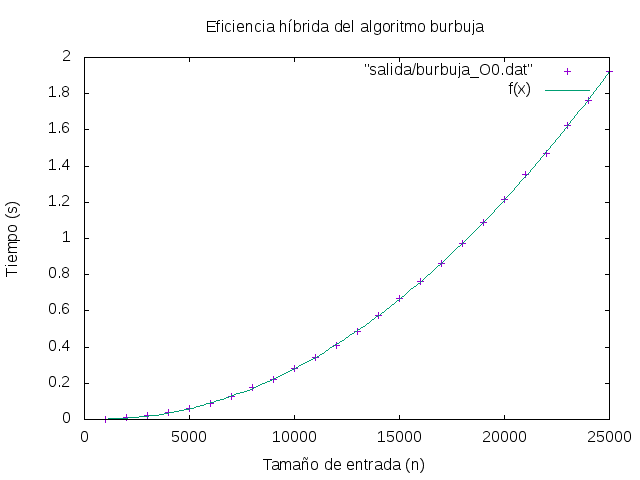
\includegraphics[clip,width=0.8\columnwidth]{../plots/burbuja_O0_fit.png}%
    \end{figure}
  \end{frame}

\begin{frame}[fragile]
  Para el ajuste he usado la función:

  $$ax^2+bx+c$$
  
\scriptsize
\begin{verbatim}
Final set of parameters            Asymptotic Standard Error
=======================            ==========================
a               = 3.28357e-09      +/- 1.726e-11    (0.5256%)
b               = -5.30415e-06     +/- 4.623e-07    (8.715%)
c               = 0.00451332       +/- 0.002608     (57.79%)
\end{verbatim}
  
\end{frame}


%
%======================
%

\begin{frame}\frametitle{Algoritmo de inserción}
  \begin{figure}[H]
    \centering   
        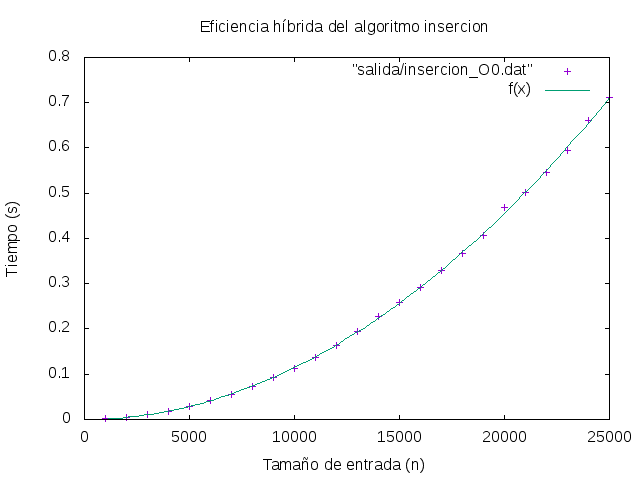
\includegraphics[clip,width=0.8\columnwidth]{../plots/insercion_O0_fit.png}%
    \end{figure}
\end{frame}

\begin{frame}[fragile]
  Para su ajuste he usado la función:

  $$ax^2+bx+c$$
  
\scriptsize
\begin{verbatim}
Final set of parameters            Asymptotic Standard Error
=======================            ==========================
a               = 1.12876e-09      +/- 1.577e-11    (1.397%)
b               = 2.22477e-07      +/- 4.225e-07    (189.9%)
c               = -0.00044311      +/- 0.002384     (538%)
\end{verbatim}

\end{frame}


%
%======================
%

\begin{frame}\frametitle{Algoritmo de selección}
  \begin{figure}[H]
    \centering   
        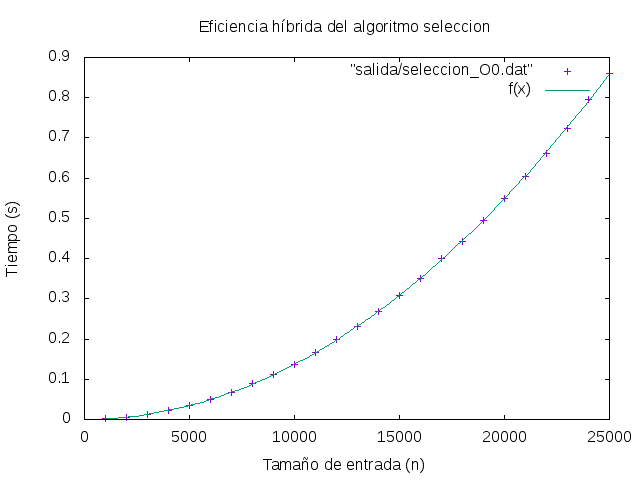
\includegraphics[clip,width=0.8\columnwidth]{../plots/seleccion_O0_fit.png}%
    \end{figure}
  \end{frame}

\begin{frame}[fragile]
  Para su ajuste he usado la función:

  $$ax^2+bx+c$$
  
\scriptsize
\begin{verbatim}
Final set of parameters            Asymptotic Standard Error
=======================            ==========================
a               = 1.37901e-09      +/- 8.147e-12    (0.5908%)
b               = -1.54865e-07     +/- 2.182e-07    (140.9%)
c               = 0.000768081      +/- 0.001231     (160.3%)
\end{verbatim}
  
\end{frame}

%
%======================
%

\begin{frame}\frametitle{Comparación de los algoritmos cuadráticos}
  \begin{figure}[H]
    \centering   
        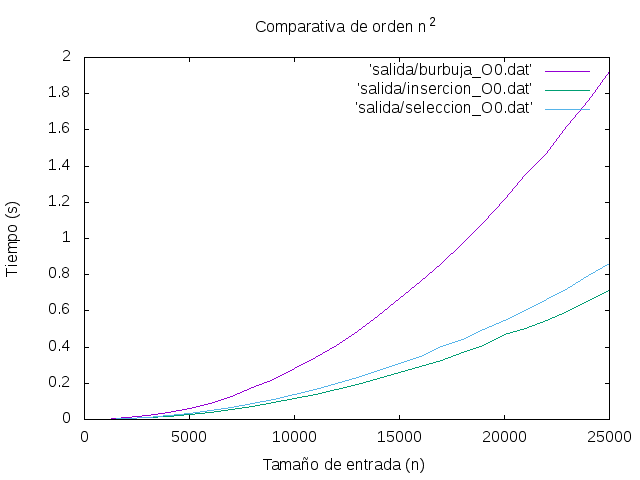
\includegraphics[clip,width=0.8\columnwidth]{../plots/cuadraticos_O0.png}%
    \end{figure}
  \end{frame}

 \begin{frame}\frametitle{Mergesort}
    \begin{figure}[H]
    \centering   
    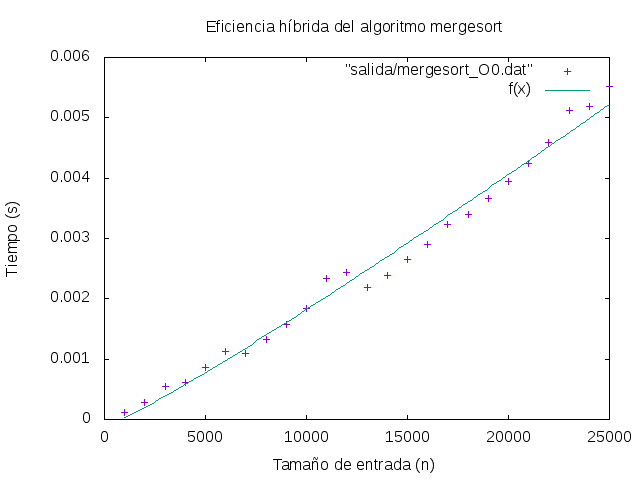
\includegraphics[clip,width=0.76\columnwidth]{../plots/mergesort_O0_fit.png}%
    \end{figure}

    Para su ajuste he usado la función: $$ex\cdot log(x)+f$$
       
  \end{frame}

   \begin{frame}\frametitle{Quicksort}
    \begin{figure}[H]
    \centering   
    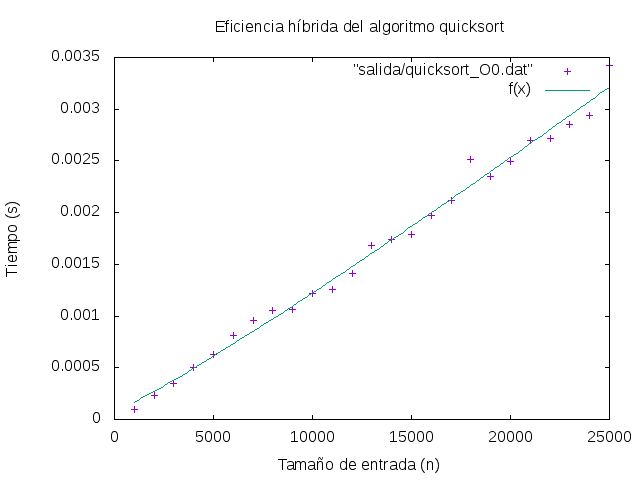
\includegraphics[clip,width=0.76\columnwidth]{../plots/quicksort_O0_fit.png}%
    \end{figure}

    Para su ajuste he usado la función: $$ex\cdot log(x)+f$$
       
  \end{frame}

   \begin{frame}\frametitle{Heapsort}
    \begin{figure}[H]
    \centering   
    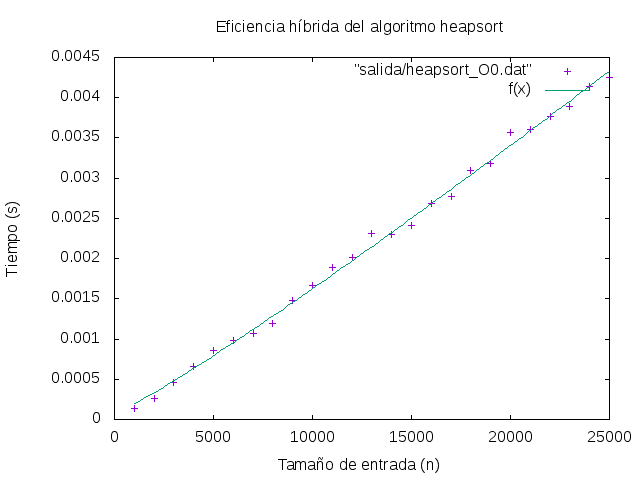
\includegraphics[clip,width=0.76\columnwidth]{../plots/heapsort_O0_fit.png}%
    \end{figure}

    Para su ajuste he usado la función: $$ex\cdot log(x)+f$$
       
  \end{frame}

\begin{frame}\frametitle{Comparación de los algoritmos n-logarítmicos}
  \begin{figure}[H]
    \centering   
        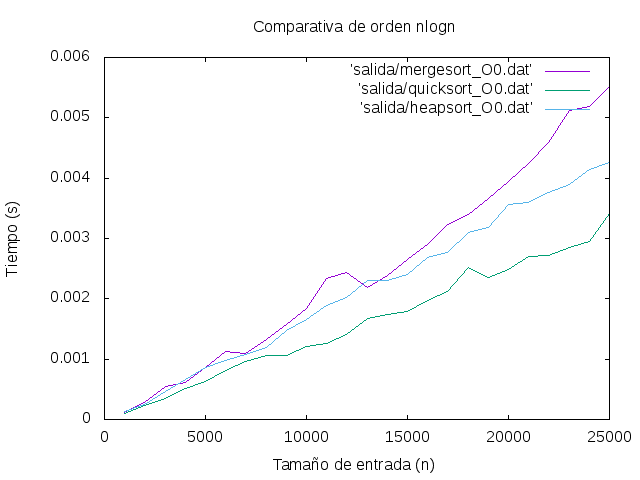
\includegraphics[clip,width=0.8\columnwidth]{../plots/logaritmicos_O0.png}%
    \end{figure}
  \end{frame}

\begin{frame}\frametitle{Floyd}
  \begin{figure}[H]
    \centering   
        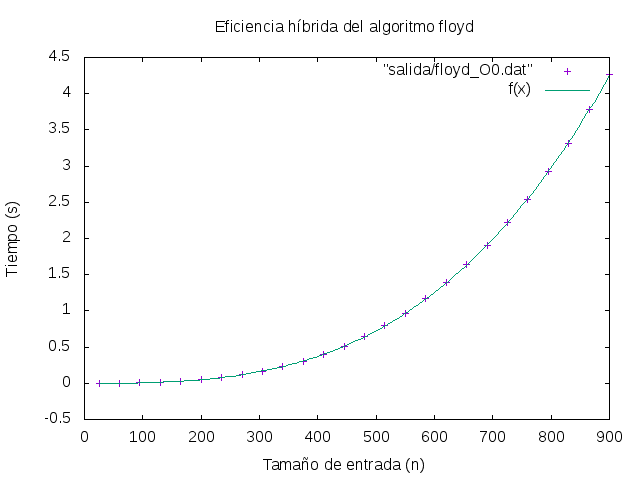
\includegraphics[clip,width=0.8\columnwidth]{../plots/floyd_O0_fit.png}%
      \end{figure}

      Ajuste realizado con la función $f(x) = ax^3 + bx^2 + cx + d$
  \end{frame}
  
  \begin{frame}\frametitle{Hanoi}
    \begin{figure}[H]
      \centering   
      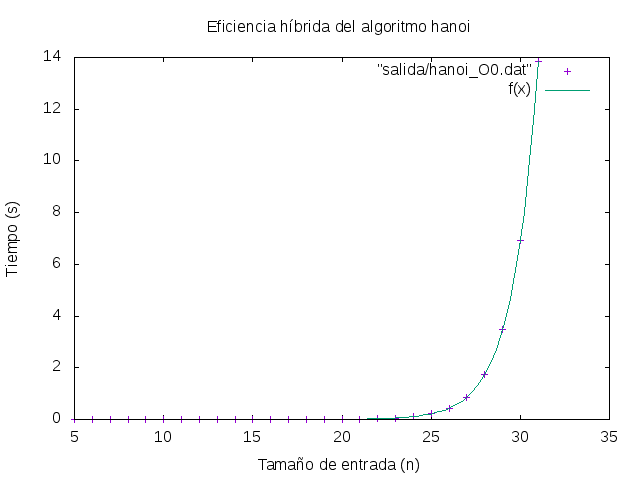
\includegraphics[clip,width=0.8\columnwidth]{../plots/hanoi_O0_fit.png}%
    \end{figure}

    Ajuste realizado con la función $a2^x$
  \end{frame}

  
\begin{frame}\frametitle{Comparaciones final}
  \begin{figure}[H]
    \centering   
        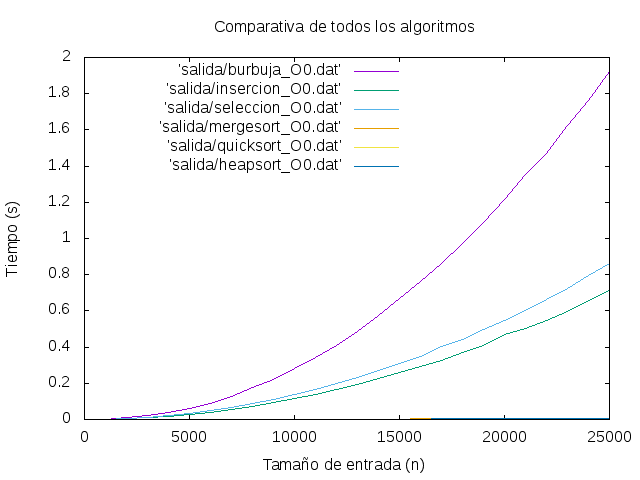
\includegraphics[clip,width=0.8\columnwidth]{../plots/todos_ordenacion_O0.png}%
      \end{figure}
  \end{frame}

\end{document}

